
% \documentclass{beamer}
\documentclass[aspectratio=169]{beamer}
% \usetheme[institute]{tugraz2013} %\ mit blauem Logo
\usetheme{tugraz2013} %\ ohne blauem Logo
% \usetheme[notes]{tugraz2013}
% \usetheme[minimal]{tugraz2013}

\title[Title]{6LoCAN \\}
\author{Alexander Wachter}
\date{\today}
\institute[Institute of Technical Informatics]{ Institute of Technical Informatics\\ Networked Embedded Systems}
\instituteurl{www.iti.tugraz.at}
%\institutelogo{iti.pdf}
% \additionallogo{institutslogo.pdf}

\usepackage[backend=biber, %% using "biber" to compile references (instead of "biblatex")
	style=numeric, 
	backref=true, %% create backlings from references to citations
	natbib=true, %% offering natbib-compatible commands
	hyperref=true, %% using hyperref-package references
	]{biblatex}  %% remove, if using BibTeX instead of biblatex

\addbibresource{references-biblatex.bib}
\usepackage{tikz}
\usetikzlibrary{positioning}

%%%%%%%%%%%%%%%%%%%%%%%%%%%%%%%%%%%%%%%%%%%%%%%%%%%%%%%%%%%%%%%%%%%%%%%%%%%%
\begin{document}
%%%%%%%%%%%%%%%%%%%%%%%%%%%%%%%%%%%%%%%%%%%%%%%%%%%%%%%%%%%%%%%%%%%%%%%%%%%%
\titleframe

\begin{frame}
  \frametitle{Content}
  \tableofcontents%[hideallsubsections] 
\end{frame}

\section{Motivation}

\begin{frame}
	\frametitle{Why do we want IPv6 on a CANbus?}
	\begin{itemize}
		\item Technology/Vendor independent
		\item Lots of application-layer protocols
		\item Transport Layer Security (TLS)
		\item Routing and access to the internet
	\end{itemize}
\end{frame}

\begin{frame}
	\frametitle{Why do we want to use CAN for IPv6?}
	\begin{itemize}
		\item Broad availability on small and large MCUs
		\item Cheap and low hardware footprint
		\item Very robust
		\item Simple wiring
		\item Widely used
	\end{itemize}
\end{frame}

\section{Introduction}
\begin{frame}
	\frametitle{CAN Bus}
	\begin{minipage}[t]{0.5\textwidth}
		\begin{itemize}
			\item Multi-Master with CSMA/CR
			\item Line topology
			\item Two-wire bus
		\end{itemize}
	\end{minipage}
	\begin{minipage}[t]{0.4\textwidth}
		\begin{table}
			\centering
			\tiny
			%\caption{Maximum bus speed}
			\begin{tabular}{|c|c|} 
				\hline
				Bus Lenght & Max. Speed \\ \hline
				[m]    & [Kbps]     \\
				\hline
				\hline
				40     & 1000       \\ \hline
				100    & 500        \\ \hline
				200    & 250        \\ \hline
				500    & 100        \\ \hline
				1000   & 50         \\ \hline
			\end{tabular}
			\label{tab:bus_speed}	
		\end{table}
	\end{minipage}
	\begin{minipage}[t]{0.05\textwidth}
		\tiny\cite{TiCANPhy}
	\end{minipage}

	\vspace{1em}
	\begin{figure}
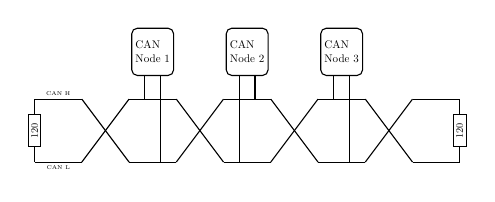
\begin{tikzpicture}[scale=0.4, every node/.style={scale=0.4}]
	\draw (0 cm, 0 cm) -- (1.5 cm, 0 cm) node[midway, below] {\tiny CAN L};
	\draw (0 cm, 2 cm) -- (1.5 cm, 2 cm) node[midway, above] {\tiny CAN H};
	\foreach \x in {3,6,9,12}{
		\draw (\x cm, 0 cm) -- (\x cm + 1.5 cm, 0 cm);
		\draw (\x cm, 2 cm) -- (\x cm + 1.5 cm, 2 cm);
	}
	\foreach \x in {1.5,4.5,7.5,10.5}{
		\draw (\x cm, 0 cm) -- (\x cm + 1.5 cm, 2 cm);
		\draw (\x cm, 2 cm) -- (\x cm + 1.5 cm, 0 cm);
	}
	\foreach \x in {0,13.5}{
		\draw (\x cm, 0 cm) -- (\x cm, 0.5 cm);
		\draw (\x cm - 0.2 cm, 0.5 cm) rectangle ++(0.4 cm,1 cm);
		\draw (\x cm, 2 cm) -- (\x cm, 1.5 cm);
		\node[rotate = 90] at (\x cm, 1cm) {\small120};
	}
	\node[draw, align=left, rounded corners=2pt, minimum height=1.5cm] (Node 1) at (3.75 cm,3.5 cm) {CAN \\Node 1};
	\draw (3.5 cm, 2cm) -- (3.5 cm, 2.75cm);
	\draw (4 cm, 0cm) -- (4 cm, 2.75cm);
	\node[draw, align=left, rounded corners=2pt, minimum height=1.5cm] (Node 2) at (6.75 cm,3.5 cm) {CAN \\Node 2};
	\draw (6.5 cm, 0cm) -- (6.5 cm, 2.75cm);
	\draw (7 cm, 2cm) -- (7 cm, 2.75cm);
	\node[draw, align=left, rounded corners=2pt, minimum height=1.5cm] (Node 2) at (9.75 cm,3.5 cm) {CAN \\Node 3};
	\draw (9.5 cm, 2cm) -- (9.5 cm, 2.75cm);
	\draw (10 cm, 0cm) -- (10 cm, 2.75cm);
\end{tikzpicture}
\end{figure}
\end{frame}

\begin{frame}
	\frametitle{CAN Frame}
	\begin{minipage}[t]{0.8\textwidth}
		\begin{itemize}
			\item 11-bit or 29-bit Identifier
			\item Up to 8 bytes payload for Classical CAN
			\item Up to 64 bytes payload for CAN-FD
		\end{itemize}
	\end{minipage}
	\begin{minipage}[t]{0.1\textwidth}
		{\tiny\cite{BoschCAN} \cite{BoschCANFD}}
	\end{minipage}

	\vspace{1.5em}
	\begin{figure}
	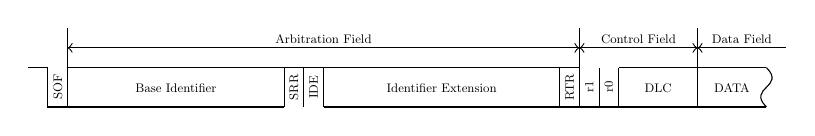
\begin{tikzpicture}[scale=0.5,  every node/.style={scale=0.5}]
		%SOF
		\draw (0,1) -- ++(0.5,0) -- ++(0,-1) -- ++(0.5,0) -- ++(0,1);
		\node[rotate=90] at (0.75,0.5) {\small SOF};
		%Base Identifier
		\draw (1,1) -- ++(5.5, 0);
		\draw (1,0) -- ++(5.5, 0) node[midway, above=0.125] {\small Base Identifier};
		\draw (6.5, 0) -- ++(0,1);
		%SRR
		\draw (6.5, 1) -- ++(0.5,0);
		\draw (7, 0) -- ++(0,1);
		\node[rotate=90] at (6.75,0.5) {\small SRR};
		%IDE
		\draw (7, 1) -- ++(0.5,0);
		\draw (7.5, 0) -- ++(0,1);
		\node[rotate=90] at (7.25,0.5) {\small IDE};
		%Identifier Extension
		\draw (7.5,1) -- ++(6, 0);
		\draw (7.5,0) -- ++(6, 0) node[midway, above=0.125] {\small Identifier Extension};
		\draw (13.5, 0) -- ++(0,1);
		%RTR
		\draw (13.5,0) -- ++(0.5,0);
		\draw (13.5,1) -- ++(0.5,0);
		\draw (14,0) -- ++(0,1);
		\node[rotate=90] at (13.75,0.5) {\small RTR};
		%R1 R0
		\draw (14,0) -- ++(1,0);
		\draw (14.5,0) -- ++(0,1);
		\node[rotate=90] at (14.25,0.5) {\small r1};
		\draw (15,0) -- ++(0,1);
		\node[rotate=90] at (14.75,0.5) {\small r0};
		%DLC
		\draw (15,1) -- ++(2,0);
		\draw (15,0) -- ++(2,0) node[midway, above=0.125] {\small DLC};
		\draw (17, 0) -- ++(0,1);
		%Data
		\draw (17,1) -- ++(1.75,0);
		\draw (17,0) -- ++(1.75,0) node[midway, above=0.125] {\small DATA};
		\draw (18.75,0) .. controls (18.25,0.5) and (19.25,0.5) .. (18.75,1);
		
		%Arbitration
		\draw (1,1) -- ++(0,1);
		\draw (14,1) -- ++(0,1);
		\draw[<->] (1,1.5) -- (14,1.5) node[midway, above] {\small Arbitration Field};
		%Control
		\draw (17,1) -- ++(0,1);
		\draw[<->] (14,1.5) -- (17,1.5) node[midway, above] {\small Control Field};
		%Data
		\draw[<-] (17,1.5) -- ++(2.25,0) node[midway, above] {\small Data Field};
		
		\end{tikzpicture}
	\end{figure}
\end{frame}

\section{Addressing}

\begin{frame}
	\frametitle{Node-Address}
	\begin{itemize}
		\item 14 bits wide
		\item Randomly or statically assigned
		\item Must be unique on the bus
	\end{itemize}
	\begin{figure}
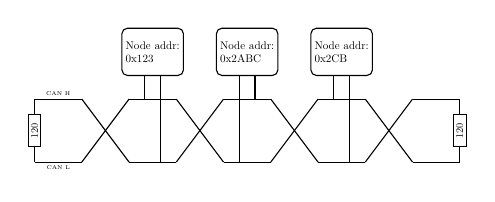
\begin{tikzpicture}[scale=0.4, every node/.style={scale=0.4}]
	\draw (0 cm, 0 cm) -- (1.5 cm, 0 cm) node[midway, below] {\tiny CAN L};
	\draw (0 cm, 2 cm) -- (1.5 cm, 2 cm) node[midway, above] {\tiny CAN H};
	\foreach \x in {3,6,9,12}{
		\draw (\x cm, 0 cm) -- (\x cm + 1.5 cm, 0 cm);
		\draw (\x cm, 2 cm) -- (\x cm + 1.5 cm, 2 cm);
	}
	\foreach \x in {1.5,4.5,7.5,10.5}{
		\draw (\x cm, 0 cm) -- (\x cm + 1.5 cm, 2 cm);
		\draw (\x cm, 2 cm) -- (\x cm + 1.5 cm, 0 cm);
	}
	\foreach \x in {0,13.5}{
		\draw (\x cm, 0 cm) -- (\x cm, 0.5 cm);
		\draw (\x cm - 0.2 cm, 0.5 cm) rectangle ++(0.4 cm,1 cm);
		\draw (\x cm, 2 cm) -- (\x cm, 1.5 cm);
		\node[rotate = 90] at (\x cm, 1cm) {\small120};
	}
	\node[draw, align=left, rounded corners=2pt, minimum height=1.5cm] (Node 1) at (3.75 cm,3.5 cm) {Node addr: \\ 0x123};
	\draw (3.5 cm, 2cm) -- (3.5 cm, 2.75cm);
	\draw (4 cm, 0cm) -- (4 cm, 2.75cm);
	\node[draw, align=left, rounded corners=2pt, minimum height=1.5cm] (Node 2) at (6.75 cm,3.5 cm) {Node addr: \\ 0x2ABC};
	\draw (6.5 cm, 0cm) -- (6.5 cm, 2.75cm);
	\draw (7 cm, 2cm) -- (7 cm, 2.75cm);
	\node[draw, align=left, rounded corners=2pt, minimum height=1.5cm] (Node 2) at (9.75 cm,3.5 cm) {Node addr: \\ 0x2CB};
	\draw (9.5 cm, 2cm) -- (9.5 cm, 2.75cm);
	\draw (10 cm, 0cm) -- (10 cm, 2.75cm);
\end{tikzpicture}
\end{figure}

\end{frame}

\begin{frame}
	\frametitle{Node-Address to Identifier}
	\begin{itemize}
		\item Bit 28 is a Multicast-flag
		\item Bit 27 down to bit 14 are the Destination Node-Address
		\item Bit 13 down to bit 0 are the Source Node-Address
	\end{itemize}
	\begin{figure}
	\begin{tikzpicture}[scale=0.35,  every node/.style={scale=0.35},
		region/.style={
			rectangle, 
			minimum height=1.5cm,
			font=\huge}]

		\node (mcast) [region, minimum width=1cm] {M};
		\node (dest) [region, right of=mcast,xshift=6.5cm, minimum width=14cm] {DEST Address};
		\node (src) [region, right of=dest,xshift=13cm, minimum width=14cm] {SRC Address};

		\draw (mcast.north west) -- (src.north east);
		\draw (mcast.south west) -- (src.south east);
		\draw (mcast.south west) -- ++(0,2.5cm);
		\draw (mcast.south east) -- ++(0,2.5cm);
		\draw (dest.south east) -- ++(0,2.5cm);
		\draw (src.south east) -- ++(0,2.5cm);
		\draw[<->] ($(mcast.north west) + (0,0.5cm)$) -- ($(mcast.north east) + (0,0.5cm)$) node[midway, above] {\large 1};
		\draw[<->] ($(mcast.north east) + (0,0.5cm)$) -- ($(dest.north east) + (0,0.5cm)$) node[midway, above] {\large 14};
		\draw[<->] ($(dest.north east) + (0,0.5cm)$) -- ($(src.north east) + (0,0.5cm)$) node[midway, above] {\large 14};
	\end{tikzpicture}
\end{figure}
\end{frame}

\begin{frame}
	\frametitle{Multicast Identifier}
	\begin{itemize}
		\item Multicast-flag is 1
		\item Destination is the lower 14 bits of the Multicast-group
	\end{itemize}
	\begin{figure}
	\begin{tikzpicture}[scale=0.35,  every node/.style={scale=0.35},
		region/.style={
			rectangle, 
			minimum height=1.5cm,
			font=\huge}]

		\node (mcast) [region, minimum width=1cm] {1};
		\node (dest) [region, right of=mcast,xshift=6.5cm, minimum width=14cm] {Multicast Group};
		\node (src) [region, right of=dest,xshift=13cm, minimum width=14cm] {SRC Address};

		\draw (mcast.north west) -- (src.north east);
		\draw (mcast.south west) -- (src.south east);
		\draw (mcast.south west) -- ++(0,2.5cm);
		\draw (mcast.south east) -- ++(0,2.5cm);
		\draw (dest.south east) -- ++(0,2.5cm);
		\draw (src.south east) -- ++(0,2.5cm);
		\draw[<->] ($(mcast.north west) + (0,0.5cm)$) -- ($(mcast.north east) + (0,0.5cm)$) node[midway, above] {\large 1};
		\draw[<->] ($(mcast.north east) + (0,0.5cm)$) -- ($(dest.north east) + (0,0.5cm)$) node[midway, above] {\large 14};
		\draw[<->] ($(dest.north east) + (0,0.5cm)$) -- ($(src.north east) + (0,0.5cm)$) node[midway, above] {\large 14};
	\end{tikzpicture}
\end{figure}
\end{frame}

\begin{frame}
	\frametitle{Link-Layer DAD}
	\begin{itemize}
		\item Send a Remote Transmission Request Frame (RTR).
			\begin{figure}
	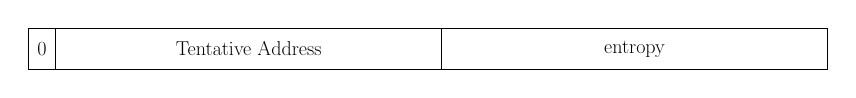
\begin{tikzpicture}[scale=0.35,  every node/.style={scale=0.35},
		region/.style={
			rectangle,
			draw=black,
			minimum height=1.5cm,
			font=\huge}]

		\node (mcast) [region, minimum width=1cm] {0};
		\node (dest) [region, right of=mcast,xshift=6.5cm, minimum width=14cm] {Tentative Address};
		\node (src) [region, right of=dest,xshift=13cm, minimum width=14cm] {entropy};
	\end{tikzpicture}
\end{figure}
		\item Wait at least 100ms for a response.
			\begin{figure}
	\begin{tikzpicture}[scale=0.35,  every node/.style={scale=0.35},
		region/.style={
			rectangle,
			draw=black,
			minimum height=1.5cm,
			font=\huge}]

		\node (mcast) [region, minimum width=1cm] {0};
		\node (dest) [region, right of=mcast,xshift=6.5cm, minimum width=14cm] {0x3DFE};
		\node (src) [region, right of=dest,xshift=13cm, minimum width=14cm] {Tentative Address};

		\draw (mcast.north west) -- (src.north east);
		\draw (mcast.south west) -- (src.south east);
		\draw (mcast.south west) -- ++(0,2.5cm);
		\draw (mcast.south east) -- ++(0,2.5cm);
		\draw (dest.south east) -- ++(0,2.5cm);
		\draw (src.south east) -- ++(0,2.5cm);
		\draw[<->] ($(mcast.north west) + (0,0.5cm)$) -- ($(mcast.north east) + (0,0.5cm)$) node[midway, above] {\large 1};
		\draw[<->] ($(mcast.north east) + (0,0.5cm)$) -- ($(dest.north east) + (0,0.5cm)$) node[midway, above] {\large 14};
		\draw[<->] ($(dest.north east) + (0,0.5cm)$) -- ($(src.north east) + (0,0.5cm)$) node[midway, above] {\large 14};

	\end{tikzpicture}
\end{figure}
	\end{itemize}	
\end{frame}


\section{Fragmentation, Reassembly and Flow-Control}

\begin{frame}
	\frametitle{Fragmentation and Reassembly}
	\begin{itemize}
		\item The minimal MTU for IPv6 is 1280 bytes
		\item CAN has 8/64 bytes
		\item ISO-TP (ISO 15765-2)
		\item Fragmentation and Reassembly
		\item Flow-Control (Unicast only)
	\end{itemize}
\end{frame}

\begin{frame}
	\begin{minipage}[t]{0.6\textwidth}
		\begin{itemize}
			\item First Frame (FF)
				\begin{itemize}
					\item Data Length
				\end{itemize}
			\item Flow-Control Frame
				\begin{itemize}
					\item Flow State (CTS, WAIT, OVFLW)
					\item Separation Time Min(ST\textsubscript{min})
					\item Block Size (BS)
				\end{itemize}
			\item Consecutive Frame
				\begin{itemize}
					\item Sequence Number
					\item Data
				\end{itemize}
		\end{itemize}
	\end{minipage}
	\begin{minipage}[t]{0.39\textwidth}
		\begin{figure}
\begin{center}
	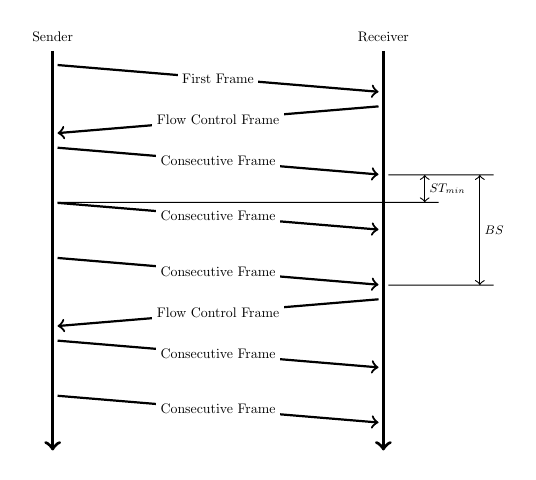
\begin{tikzpicture}[scale=0.35, every node/.style={scale=0.5}]
		%Sender
		\node (s_ff) at (0,14)  {};
		\node (s_fc1) at (0,11.5) {};
		\node (s_cf1) at (0,11) {};
		\node (s_cf2) at (0,9) {};
		\node (s_cf3) at (0,7) {};
		\node (s_fc2) at (0,4.5) {};
		\node (s_cf4) at (0,4) {};
		\node (s_cf5) at (0,2) {};
		
		%Receiver
		\node (r_ff) at (12,13)  {};
		\node (r_fc1) at (12,12.5) {};
		\node (r_cf1) at (12,10) {};
		\node (r_cf2) at (12,8) {};
		\node (r_cf3) at (12,6) {};
		\node (r_fc2) at (12,5.5) {};
		\node (r_cf4) at (12,3) {};
		\node (r_cf5) at (12,1) {};

		%connections
		\draw[thick, ->] (s_ff) -- node[midway, fill=white] {First Frame} (r_ff);
		\draw[thick,->] (r_fc1) -- node[midway, fill=white] {Flow Control Frame} (s_fc1);
		\draw[thick,->] (s_cf1) -- node[midway, fill=white] {Consecutive Frame} (r_cf1);
		\draw[thick,->] (s_cf2) -- node[midway, fill=white] {Consecutive Frame} (r_cf2);
		\draw[thick,->] (s_cf3) -- node[midway, fill=white] {Consecutive Frame} (r_cf3);
		\draw[thick,->] (r_fc2) -- node[midway, fill=white] {Flow Control Frame} (s_fc2);
		\draw[thick,->] (s_cf4) -- node[midway, fill=white] {Consecutive Frame} (r_cf4);
		\draw[thick,->] (s_cf5) -- node[midway, fill=white] {Consecutive Frame} (r_cf5);
		
		%stmin
		\draw (r_cf1) -- ++(4,0);
		\draw (s_cf2) -- ++(14,0);
		\draw[<->] (13.5,9) -- (13.5,10) node[midway,right]{\small $ST_{min}$};
		\draw (r_cf3) -- ++(4,0);
		\draw[<->] (15.5,6) -- (15.5,10) node[midway,right]{\small $BS$};
		
		%Flow
		\draw[very thick, ->] (0,14.5) --  (0,0);
		\node at (0,15) {Sender};
		\draw[very thick, ->] (12,14.5) -- (12,0);
		\node at (12,15) {Receiver};
		
	\end{tikzpicture}
\end{center}
\end{figure}
	\end{minipage}
\end{frame}

\begin{frame}
	\frametitle{6lo IPHC}
	\begin{itemize}
		\item IPv6 header has 40 bytes (six CAN frames)
		\item To bulky for CAN
		\item 6lo IPHC for Header Compression
	\end{itemize}
\end{frame}

\begin{frame}
	\frametitle{Frame Format}
	\begin{figure}
	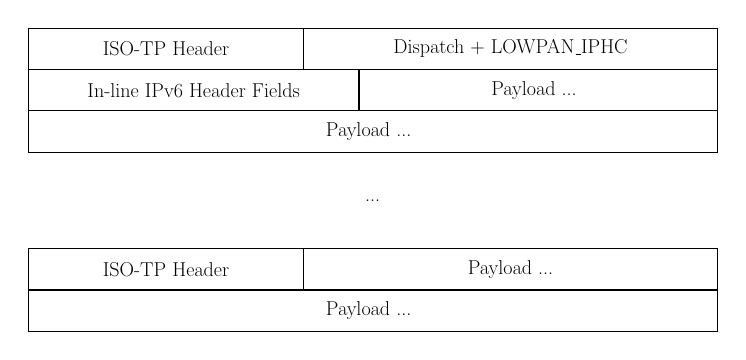
\begin{tikzpicture}[scale=0.35,  every node/.style={scale=0.35},
		region/.style={
			minimum height=1.5cm,
			align=left,
			draw,
			font=\huge}]

		\node (isotp) [region, anchor=west, minimum width=10cm] {ISO-TP Header};
		\node (iphc) [region, right of = isotp, xshift=11.5cm, minimum width=15cm] {Dispatch + LOWPAN\_IPHC};
		\node (inline) [region,anchor=west, yshift=-1.5cm, minimum width=12cm] {In-line IPv6 Header Fields};
		\node (payload) [region, right of=inline, xshift=11.5cm, minimum width=13cm] {Payload ... };
		\node (dayload2) [region,anchor=west, yshift=-3cm, minimum width=25cm] {Payload ... };

		\node at (12.5cm, -5.5cm) {\huge ...};

		\node (isotp2) [region, anchor=west, yshift=-8cm, minimum width=10cm] {ISO-TP Header};
		\node (iphc3) [region, right of = isotp2, xshift=11.5cm, minimum width=15cm] {Payload ...};
		\node (dayload4) [region,anchor=west, yshift=-9.5cm, minimum width=25cm] {Payload ... };
	\end{tikzpicture}
\end{figure}
\end{frame}

\section{Border Translator}
\begin{frame}
	\frametitle{Border Translator}
	\begin{figure}
	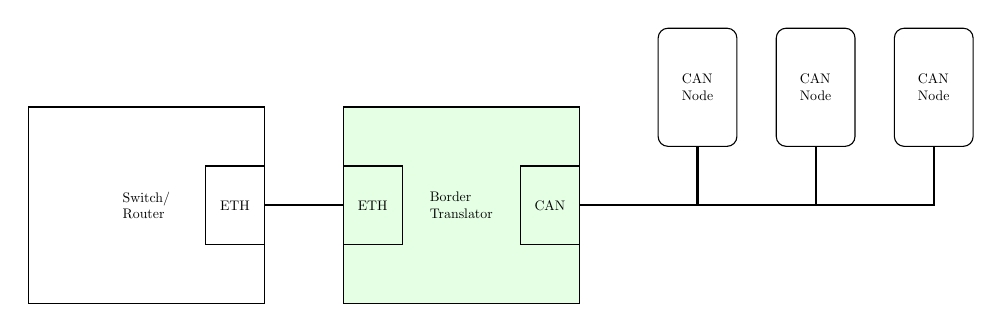
\begin{tikzpicture}[scale=0.5,  every node/.style={scale=0.5},
		rect/.style={
			draw,
            minimum height=5cm,
            minimum width=6cm,
            align=left},
            iface/.style={
			draw,
            minimum height=2cm,
            minimum width=1.5cm},
            can/.style={
            draw,
            align=left,
            minimum height=3cm,
            minimum width=2cm,
            rounded corners=0.125cm}]

        \node (switch) [rect] {Switch/ \\Router};
        \node (switchEth) [iface, right of = switch, xshift=1.25cm] {ETH};

      
        \node (bt) [rect, fill=green!10, right of = switch, xshift=7cm] {Border \\Translator};
        \node (bteth) [iface, left of = bt, xshift=-1.25cm] {ETH};
        \node (btcan) [iface, right of = bt, xshift=1.25cm] {CAN};

        \node (can1) [can, right of = bt, xshift=5cm, yshift=3cm] {CAN \\Node};
        \node (can2) [can, right of = can1, xshift=2cm] {CAN \\Node};
        \node (can3) [can, right of = can2, xshift=2cm] {CAN \\Node};

        \draw [thick] (switchEth) -- (bteth);
        \draw [thick] (btcan) -| (can1);
        \draw [thick] (btcan) -| (can2);
        \draw [thick] (btcan) -| (can3);

	\end{tikzpicture}
\end{figure}
\end{frame}

\begin{frame}
	\frametitle{Border Translator}
	\begin{itemize}
		\item Fixed Node-Address (0x3DF0)
		\item Ethernet MAC-Address is inlined
	\end{itemize}
	\begin{figure}
	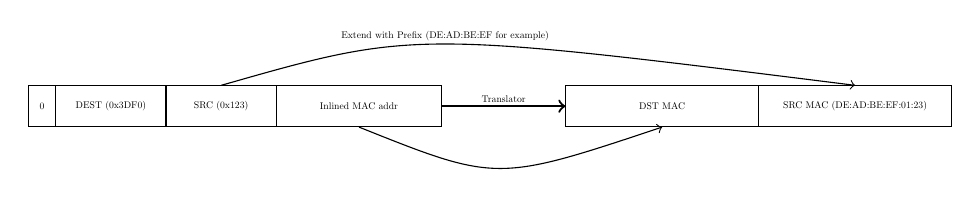
\begin{tikzpicture}[scale=0.35,  every node/.style={scale=0.35},
		region/.style={
			rectangle,
			draw,
			minimum height=1.5cm}]

		\node (mcast) [region, minimum width=1cm] {0};
		\node (dest) [region, right of=mcast,xshift=1.5cm, minimum width=4cm] { DEST (0x3DF0)};
		\node (src) [region, right of=dest,xshift=3cm, minimum width=4cm] {SRC (0x123)};
		\node (dstmacil) [region, right of=src,xshift=4cm, minimum width=6cm] {Inlined MAC addr};

		\node (dstmac) [region, right of=dstmacil, xshift=10cm, minimum width=7cm] {DST MAC};
		\node (srcmac) [region, right of=dstmac, xshift=6cm, minimum width=7cm] {SRC MAC (DE:AD:BE:EF:01:23)};

		\draw[thick, ->] (dstmacil.east) -- (dstmac.west) node [midway, above] {Translator};
		\draw[->] (dstmacil.south) .. controls ++(5cm,-2cm) .. (dstmac.south);
		\draw[->] (src.north) .. controls ++(7cm,2cm) .. (srcmac.north) node [midway, above] {Extend with Prefix (DE:AD:BE:EF for example)};
	\end{tikzpicture}
\end{figure}
\end{frame}

\begin{frame}
	\frametitle{Border Translator}
	\begin{itemize}
		\item Fixed Node-Address (0x3DF0)
		\item Ethernet MAC-Address is inlined
	\end{itemize}
	\begin{figure}
	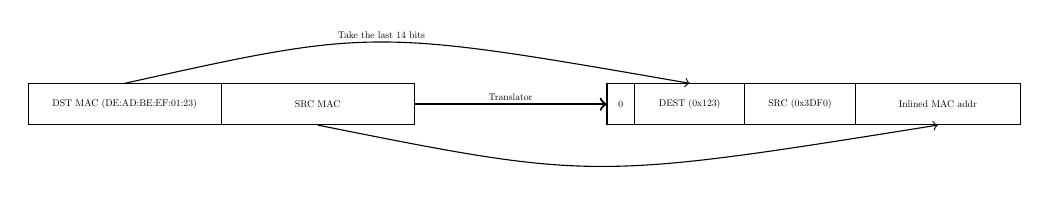
\begin{tikzpicture}[scale=0.35,  every node/.style={scale=0.35},
		region/.style={
			rectangle,
			draw,
			minimum height=1.5cm}]

		\node (dstmac) [region,, minimum width=7cm] {DST MAC (DE:AD:BE:EF:01:23)};
		\node (srcmac) [region, right of=dstmac, xshift=6cm, minimum width=7cm] {SRC MAC};

		\node (mcast) [region,right of=srcmac, xshift=10cm, minimum width=1cm] {0};
		\node (dest) [region, right of=mcast,xshift=1.5cm, minimum width=4cm] {DEST (0x123)};
		\node (src) [region, right of=dest,xshift=3cm, minimum width=4cm] {SRC (0x3DF0)};
		\node (dstmacil) [region, right of=src,xshift=4cm, minimum width=6cm] {Inlined MAC addr};

		\draw[thick, ->] (srcmac.east) -- (mcast.west) node [midway, above] {Translator};
		\draw[->] (srcmac.south) .. controls ++(10cm,-2cm) .. (dstmacil.south);
		\draw[->] (dstmac.north) .. controls ++(9cm,2cm) .. (dest.north) node [midway, above] {Take the last 14 bits};
	\end{tikzpicture}
\end{figure}
\end{frame}

\section{Reference Implementation}
\begin{frame}
	\frametitle{Reference Implementation}
	\begin{minipage}[t]{0.6\textwidth}
		\begin{itemize}
			\item Zephyr RTOS (zephyrproject.org)
			\item Since version 2.0
		\end{itemize}
	\end{minipage}
	\begin{minipage}[t]{0.39\textwidth}
		
\includegraphics[width=0.9\textwidth]{figures/Zephyr-Project.png}
	\end{minipage}
\end{frame}

\section{}

\begin{frame}
	\frametitle{ }
	\vspace{40pt}
	{\Huge Thank you. \\ Questions?} \\
	\vspace{10pt}
	Please provide feedback. \\
	\vspace{20pt}
	https://tools.ietf.org/html/draft-wachter-6lo-can-00 \\
	https://www.zephyrproject.org/
\end{frame}

\section{References}
\begin{frame}
	\frametitle{References}
	\printbibliography
\end{frame}
%%%%%%%%%%%%%%%%%%%%%%%%%%%%%%%%%%%%%%%%%%%%%%%%%%%%%%%%%%%%%%%%%%%%%%%%%%%%
\end{document}
%%%%%%%%%%%%%%%%%%%%%%%%%%%%%%%%%%%%%%%%%%%%%%%%%%%%%%%%%%%%%%%%%%%%%%%%%%%%
